\documentclass{standalone}
\usepackage{tikz}
\usetikzlibrary{patterns, positioning}
\usepackage[sfdefault]{ClearSans} %% option 'sfdefault' activates Clear Sans as the default text font
\usepackage[T1]{fontenc}

\begin{document}
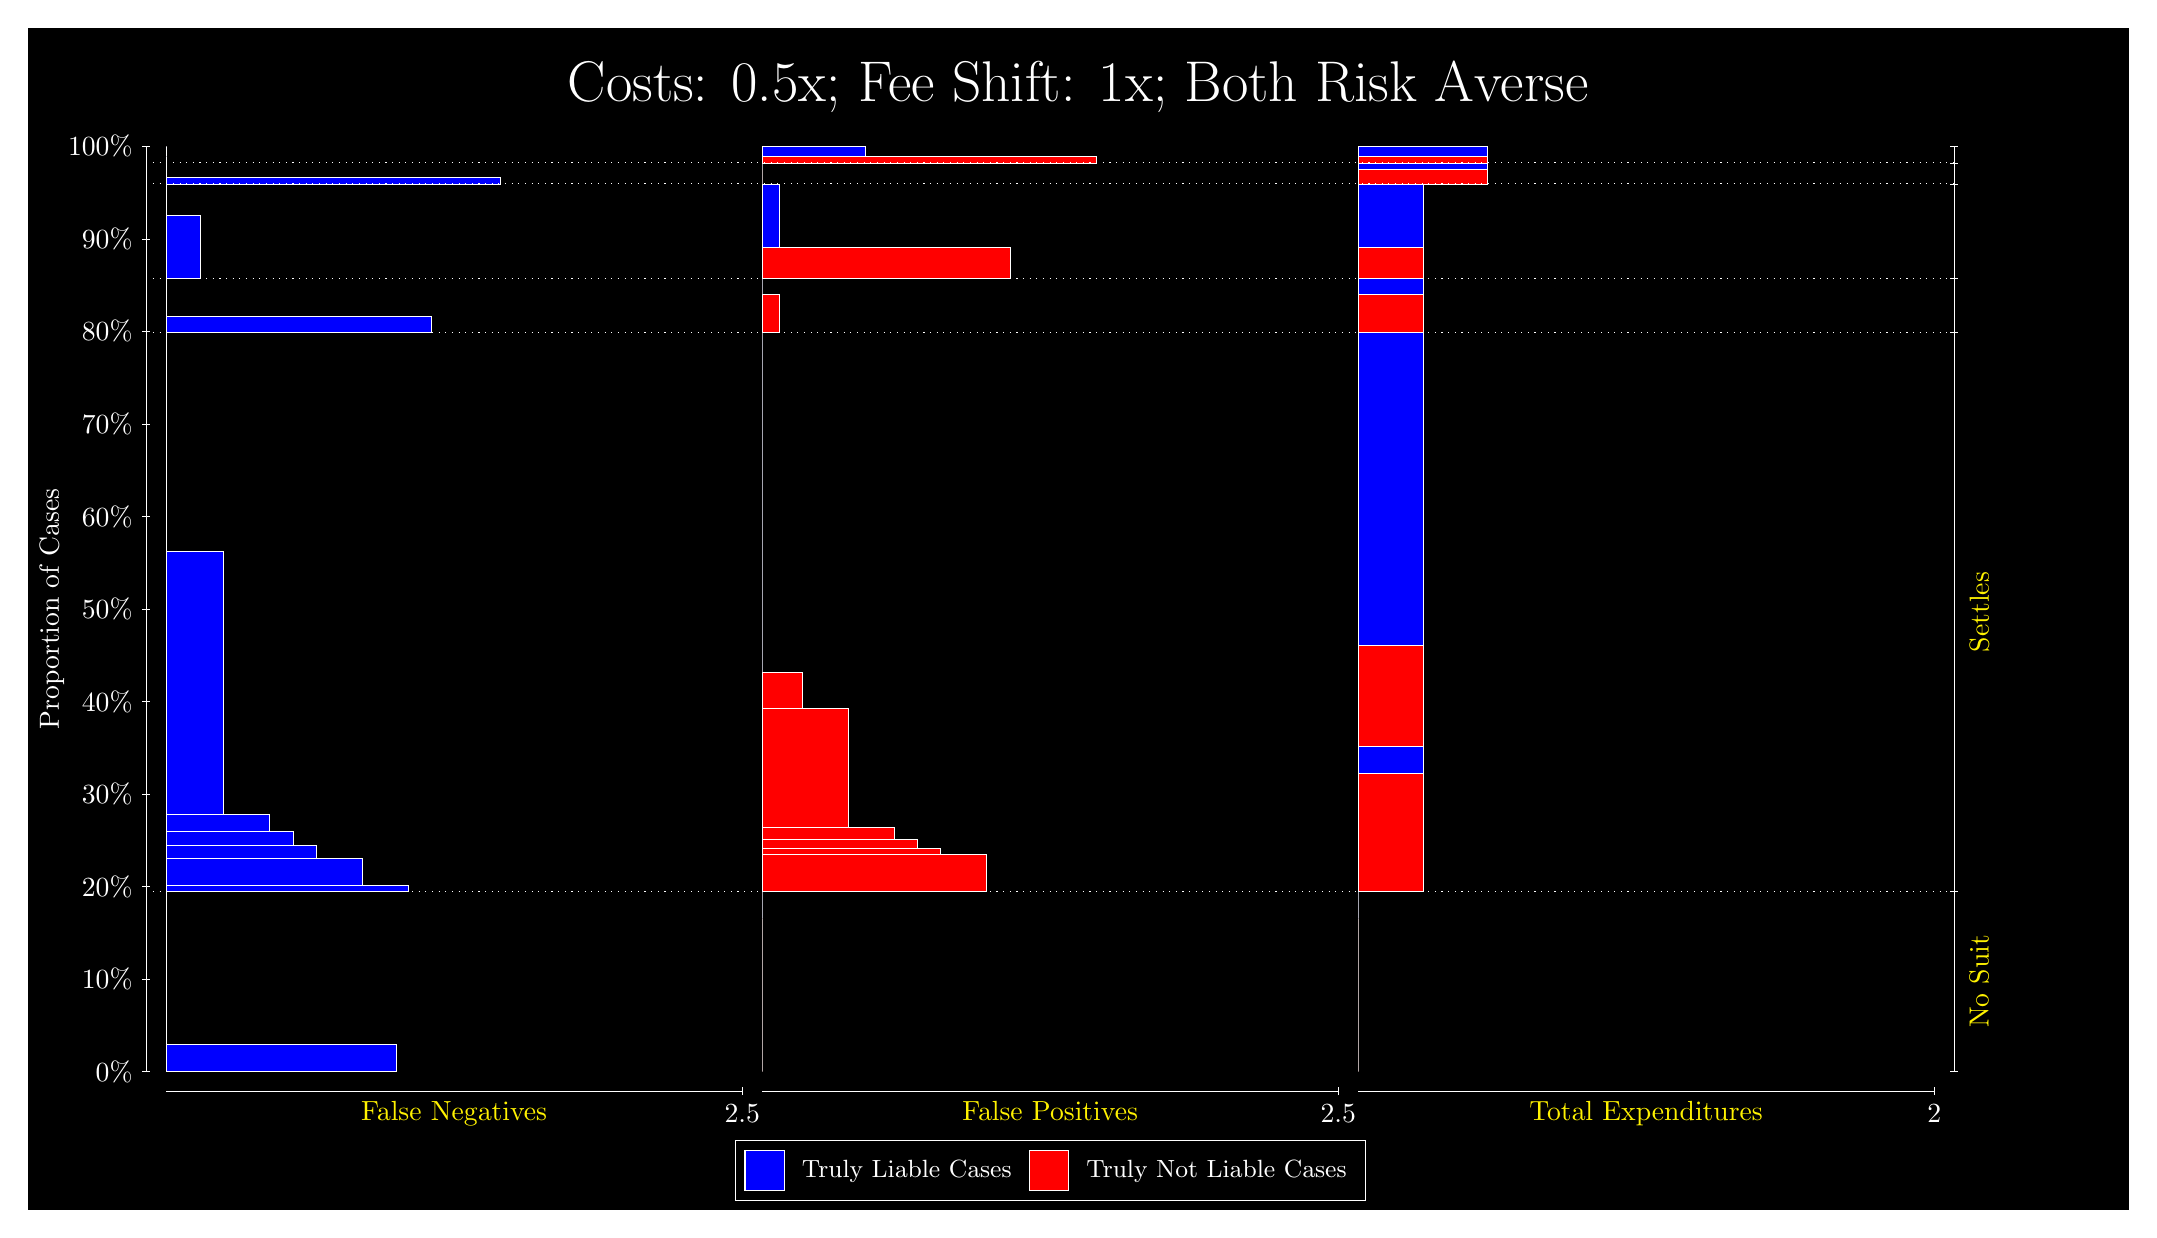
\begin{tikzpicture}
\draw[fill=black] (0,0) rectangle (26.667,15);
\draw[text=white] (0,13.5) rectangle (26.667,15) node[midway] {\huge Costs: 0.5x; Fee Shift: 1x; Both Risk Averse};
\draw[white, very thin] (1.5,1.75) -- (1.5,13.5);
\node[rotate=90, text=white, anchor=center] at (0.3, 7.625) {Proportion of Cases};
\draw[white, very thin] (1.45,1.75) -- (1.55,1.75);
\node[text=white, anchor=east] at (1.45, 1.75) {0\%};
\draw[white, very thin] (1.45,2.925) -- (1.55,2.925);
\node[text=white, anchor=east] at (1.45, 2.925) {10\%};
\draw[white, very thin] (1.45,4.1) -- (1.55,4.1);
\node[text=white, anchor=east] at (1.45, 4.1) {20\%};
\draw[white, very thin] (1.45,5.275) -- (1.55,5.275);
\node[text=white, anchor=east] at (1.45, 5.275) {30\%};
\draw[white, very thin] (1.45,6.45) -- (1.55,6.45);
\node[text=white, anchor=east] at (1.45, 6.45) {40\%};
\draw[white, very thin] (1.45,7.625) -- (1.55,7.625);
\node[text=white, anchor=east] at (1.45, 7.625) {50\%};
\draw[white, very thin] (1.45,8.8) -- (1.55,8.8);
\node[text=white, anchor=east] at (1.45, 8.8) {60\%};
\draw[white, very thin] (1.45,9.975) -- (1.55,9.975);
\node[text=white, anchor=east] at (1.45, 9.975) {70\%};
\draw[white, very thin] (1.45,11.15) -- (1.55,11.15);
\node[text=white, anchor=east] at (1.45, 11.15) {80\%};
\draw[white, very thin] (1.45,12.325) -- (1.55,12.325);
\node[text=white, anchor=east] at (1.45, 12.325) {90\%};
\draw[white, very thin] (1.45,13.5) -- (1.55,13.5);
\node[text=white, anchor=east] at (1.45, 13.5) {100\%};

\draw[white, very thin] (24.457,1.75) -- (24.457,13.5);
\draw[white, very thin] (24.407,1.75) -- (24.507,1.75);
\node[anchor=west] at (24.407, 1.75) {};
\draw[white, very thin] (24.407,4.0394) -- (24.507,4.0394);
\node[anchor=west] at (24.407, 4.0394) {};
\draw[white, very thin] (24.407,11.134) -- (24.507,11.134);
\node[anchor=west] at (24.407, 11.134) {};
\draw[white, very thin] (24.407,11.823) -- (24.507,11.823);
\node[anchor=west] at (24.407, 11.823) {};
\draw[white, very thin] (24.407,13.024) -- (24.507,13.024);
\node[anchor=west] at (24.407, 13.024) {};
\draw[white, very thin] (24.407,13.291) -- (24.507,13.291);
\node[anchor=west] at (24.407, 13.291) {};
\draw[white, very thin] (24.407,13.5) -- (24.507,13.5);
\node[anchor=west] at (24.407, 13.5) {};

\draw[white, very thin, fill=blue] (1.75,1.75) rectangle (4.6775,2.0953);
\draw[white, very thin, fill=red] (1.75,2.0953) rectangle (1.75,4.0394);
\draw[white, very thin, fill=blue] (1.75,4.0394) rectangle (4.8239,4.1128);
\draw[white, very thin, fill=blue] (1.75,4.1128) rectangle (4.2384,4.4545);
\draw[white, very thin, fill=blue] (1.75,4.4545) rectangle (3.6529,4.6225);
\draw[white, very thin, fill=blue] (1.75,4.6225) rectangle (3.3602,4.8027);
\draw[white, very thin, fill=blue] (1.75,4.8027) rectangle (3.0674,5.0186);
\draw[white, very thin, fill=blue] (1.75,5.0186) rectangle (2.4819,8.3514);
\draw[white, very thin, fill=red] (1.75,8.3514) rectangle (1.75,11.134);
\draw[white, very thin, fill=blue] (1.75,11.134) rectangle (5.1167,11.339);
\draw[white, very thin, fill=red] (1.75,11.339) rectangle (1.75,11.823);
\draw[white, very thin, fill=blue] (1.75,11.823) rectangle (2.1891,12.627);
\draw[white, very thin, fill=red] (1.75,12.627) rectangle (1.75,13.024);
\draw[white, very thin, fill=blue] (1.75,13.024) rectangle (5.9949,13.103);
\draw[white, very thin, fill=red] (1.75,13.103) rectangle (1.75,13.291);
\draw[white, very thin, fill=red] (1.75,13.291) rectangle (1.75,13.371);
\draw[white, very thin, fill=blue] (1.75,13.371) rectangle (1.75,13.5);
\draw[white, very thin, fill=red] (9.3189,1.75) rectangle (9.3189,3.6941);
\draw[white, very thin, fill=blue] (9.3189,3.6941) rectangle (9.3189,4.0394);
\draw[white, very thin, fill=red] (9.3189,4.0394) rectangle (12.173,4.5117);
\draw[white, very thin, fill=red] (9.3189,4.5117) rectangle (11.588,4.5874);
\draw[white, very thin, fill=red] (9.3189,4.5874) rectangle (11.295,4.6983);
\draw[white, very thin, fill=red] (9.3189,4.6983) rectangle (11.002,4.8555);
\draw[white, very thin, fill=red] (9.3189,4.8555) rectangle (10.417,6.3583);
\draw[white, very thin, fill=red] (9.3189,6.3583) rectangle (9.8312,6.822);
\draw[white, very thin, fill=blue] (9.3189,6.822) rectangle (9.3189,11.134);
\draw[white, very thin, fill=red] (9.3189,11.134) rectangle (9.5384,11.619);
\draw[white, very thin, fill=blue] (9.3189,11.619) rectangle (9.3189,11.823);
\draw[white, very thin, fill=red] (9.3189,11.823) rectangle (12.466,12.22);
\draw[white, very thin, fill=blue] (9.3189,12.22) rectangle (9.5384,13.024);
\draw[white, very thin, fill=red] (9.3189,13.024) rectangle (9.3189,13.211);
\draw[white, very thin, fill=blue] (9.3189,13.211) rectangle (9.3189,13.291);
\draw[white, very thin, fill=red] (9.3189,13.291) rectangle (13.564,13.371);
\draw[white, very thin, fill=blue] (9.3189,13.371) rectangle (10.636,13.5);
\draw[white, very thin, fill=red] (16.888,1.75) rectangle (16.888,3.6941);
\draw[white, very thin, fill=blue] (16.888,3.6941) rectangle (16.888,4.0394);
\draw[white, very thin, fill=red] (16.888,4.0394) rectangle (17.711,5.5423);
\draw[white, very thin, fill=blue] (16.888,5.5423) rectangle (17.711,5.884);
\draw[white, very thin, fill=red] (16.888,5.884) rectangle (17.711,7.1637);
\draw[white, very thin, fill=blue] (16.888,7.1637) rectangle (17.711,11.134);
\draw[white, very thin, fill=red] (16.888,11.134) rectangle (17.711,11.619);
\draw[white, very thin, fill=blue] (16.888,11.619) rectangle (17.711,11.823);
\draw[white, very thin, fill=red] (16.888,11.823) rectangle (17.711,12.22);
\draw[white, very thin, fill=blue] (16.888,12.22) rectangle (17.711,13.024);
\draw[white, very thin, fill=red] (16.888,13.024) rectangle (18.534,13.211);
\draw[white, very thin, fill=blue] (16.888,13.211) rectangle (18.534,13.291);
\draw[white, very thin, fill=red] (16.888,13.291) rectangle (18.534,13.371);
\draw[white, very thin, fill=blue] (16.888,13.371) rectangle (18.534,13.5);
\draw[white, dotted] (1.5,4.0394) -- (24.457,4.0394);
\draw[white, dotted] (1.5,11.134) -- (24.457,11.134);
\draw[white, dotted] (1.5,11.823) -- (24.457,11.823);
\draw[white, dotted] (1.5,13.024) -- (24.457,13.024);
\draw[white, dotted] (1.5,13.291) -- (24.457,13.291);
\draw[white, very thin] (1.75,1.5) -- (9.0689,1.5);
\node[text=yellow, anchor=north] at (5.4094, 1.5) {False Negatives};
\draw[white, very thin] (9.0689,1.45) -- (9.0689,1.55);
\node[text=white, anchor=north] at (9.0689, 1.45) {2.5};

\draw[white, very thin] (9.3189,1.5) -- (16.638,1.5);
\node[text=yellow, anchor=north] at (12.978, 1.5) {False Positives};
\draw[white, very thin] (16.638,1.45) -- (16.638,1.55);
\node[text=white, anchor=north] at (16.638, 1.45) {2.5};

\draw[white, very thin] (16.888,1.5) -- (24.207,1.5);
\node[text=yellow, anchor=north] at (20.547, 1.5) {Total Expenditures};
\draw[white, very thin] (24.207,1.45) -- (24.207,1.55);
\node[text=white, anchor=north] at (24.207, 1.45) {2};

\node[text=yellow, centered, rotate=90] at (24.777, 2.8947) {No Suit};
\node[text=yellow, centered, rotate=90] at (24.777, 7.5867) {Settles};





\draw (12.978300999999998,1.5) node[draw=none] (baseCoordinate) {};
\begin{scope}[align=center]
        \matrix[scale=0.5, draw=white, below=0.5cm of baseCoordinate, nodes={draw}, column sep=0.1cm]{
            \node[rectangle, draw, minimum width=0.5cm, minimum height=0.5cm, fill=blue] {}; &
            \node[draw=none, font=\small, text=white] (B) {Truly Liable Cases}; &
            \node[rectangle, draw, minimum width=0.5cm, minimum height=0.5cm, fill=red] {}; &
            \node[draw=none, font=\small, text=white] (B) {Truly Not Liable Cases}; \\
            };
\end{scope}

\end{tikzpicture}
\end{document}